\documentclass{article}
%\usepackage{geometry}
% \geometry{top = 1in, bottom = 1in, left = 1in, right = 1in}
\usepackage[top = 0.7in, bottom = 0.7in, left = 0.7in, right = 0.7in]{geometry}

\usepackage{amsmath,amssymb,amsthm,mathrsfs}

\usepackage{graphicx}

\usepackage{bm}
\usepackage{float}
\usepackage[font=footnotesize,labelfont=bf]{caption}


\usepackage{fancyhdr}
\pagestyle{fancy}
\rhead{\footnotesize {07/30/2012 ; MESA version 4161} }
\chead{\footnotesize {Authors: Jared Brooks, Lars Bildsten, Bill Paxton} }
\lhead{\footnotesize {mesa/star/test\_suite/very\_low\_mass} }

\begin{document}

	\begin{center}
		\begin{Large}
			\textbf{VERY LOW MASS}\\
		\end{Large}
	\end{center}

        This test is to show how \texttt{MESA} can handle stars with very low mass.  If everything ran successfully, the run should be cut off when the star's age reaches 10 Gyr (\texttt{max\_age = 10d9}).\\

        This test case loads a pre-saved model of a 0.001 $M_\odot$ brown dwarf.  The brown dwarf stays fully convective throughout the entire evolution, and, therefore, the abundances of the elements (figure \ref{fig:1}), given in log mass fraction, are constant in q, where q is the fraction of star mass interior to outer boundary of each zone, moving outward fromt the core.

	\begin{figure}[H]
		\centering
		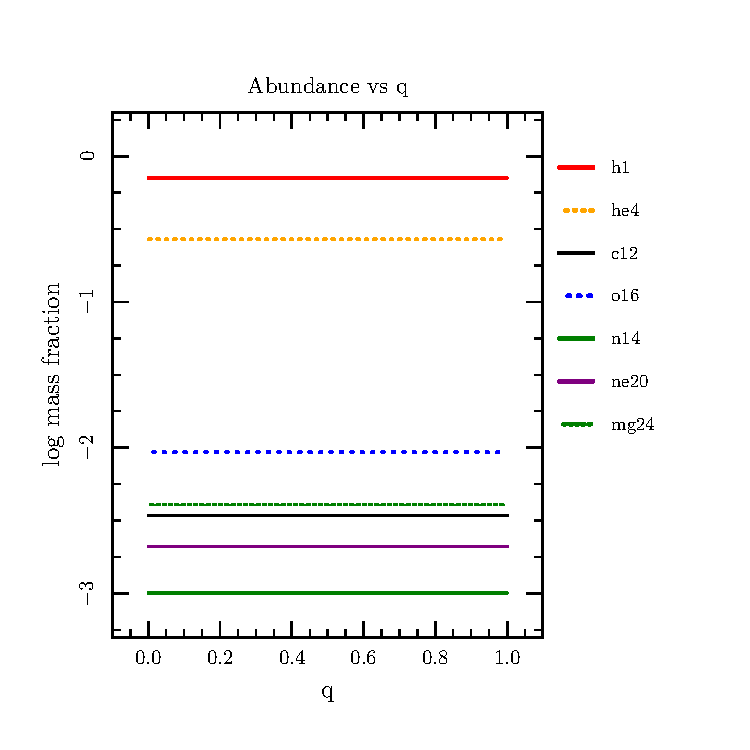
\includegraphics[width = 5in]{/Users/jaredbrooks/very_low_mass/plots_out/Abundance_vs_q_3.pdf}
		\caption{Abundance profile}
		\label{fig:1}
	\end{figure}

        \pagebreak

        The effective temperature (figure \ref{fig:2}) and radius evolution (figure \ref{fig:3}) are shown in the two plots below.

        \begin{figure}[H]
                \begin{minipage}[b]{0.5\linewidth}
                       \centering
                       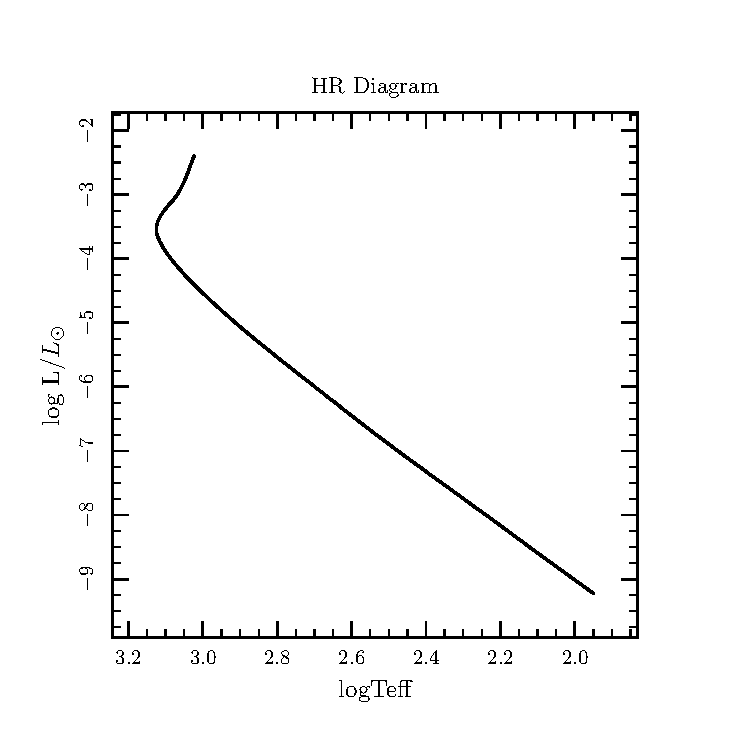
\includegraphics[width = 3.65in]{/Users/jaredbrooks/very_low_mass/plots_out/HR_Diagram.pdf}
                       \caption{\footnotesize HR-diagram where the evolution track goes from top to bottom}
                       \label{fig:2}
                \end{minipage}
                \hspace{0cm}
                \begin{minipage}[b]{0.5\linewidth}
                       \centering
                       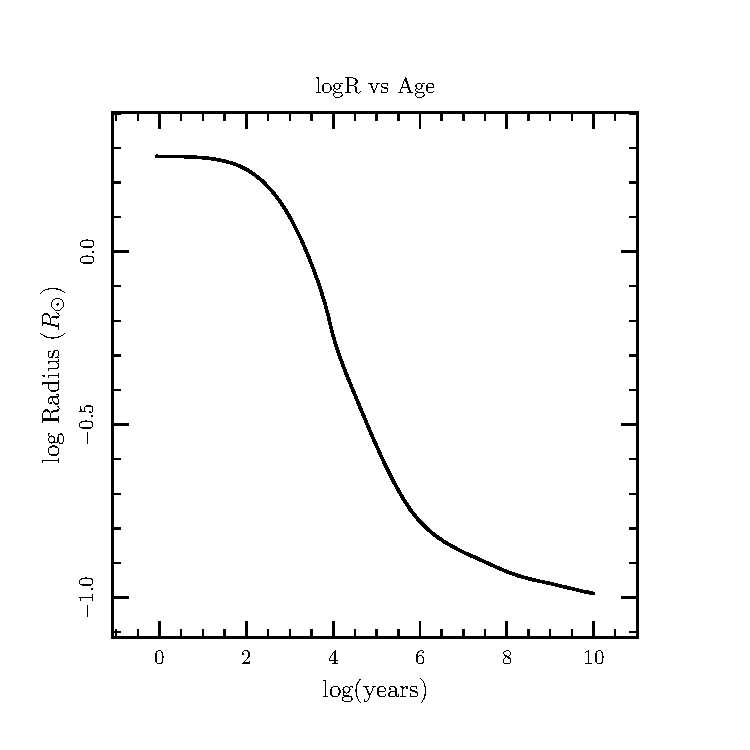
\includegraphics[width = 3.65in]{/Users/jaredbrooks/very_low_mass/plots_out/logR_vs_log_Age.pdf}
                       \caption{\footnotesize Gravitational potential energy is released as the star contracts, leading to slight rise in effective temperature}
                       \label{fig:3}
                \end{minipage}
        \end{figure}

        This next plot to the left (figure \ref{fig:4}) similarly shows effective temperature behavior, but against log[g], and a profile of temperature vs. density at a few diffent ages (figure \ref{fig:5}).

        \begin{figure}[H]
                \begin{minipage}{0.5\linewidth}
                       \centering
                       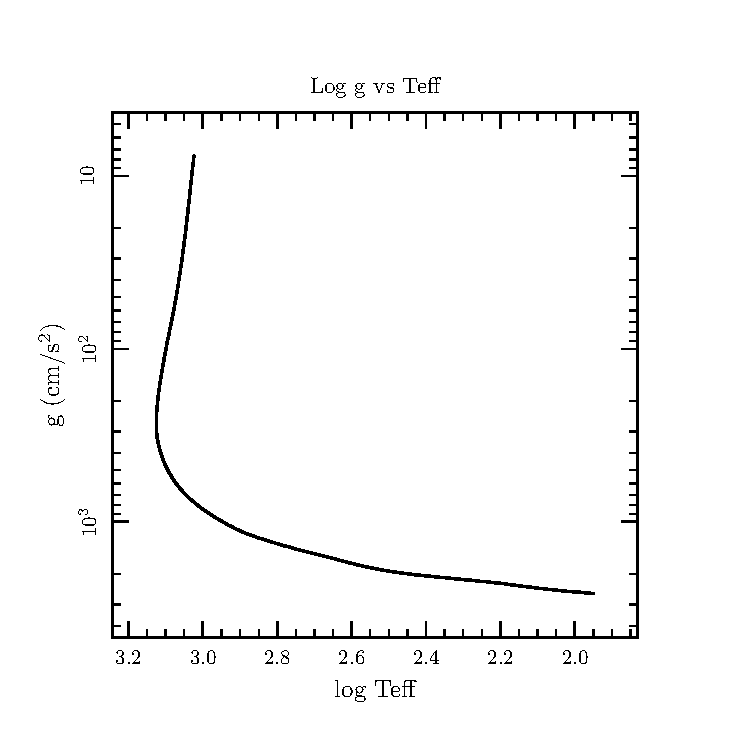
\includegraphics[width = 3.65in]{/Users/jaredbrooks/very_low_mass/plots_out/log_g_vs_Teff.pdf}
                       \caption{\footnotesize Log g vs. effective T where the evolution track goes from top to bottom}
                       \label{fig:4}
                       \end{minipage}
                \hspace{0cm}
                \begin{minipage}{0.5\linewidth}
                       \centering
                       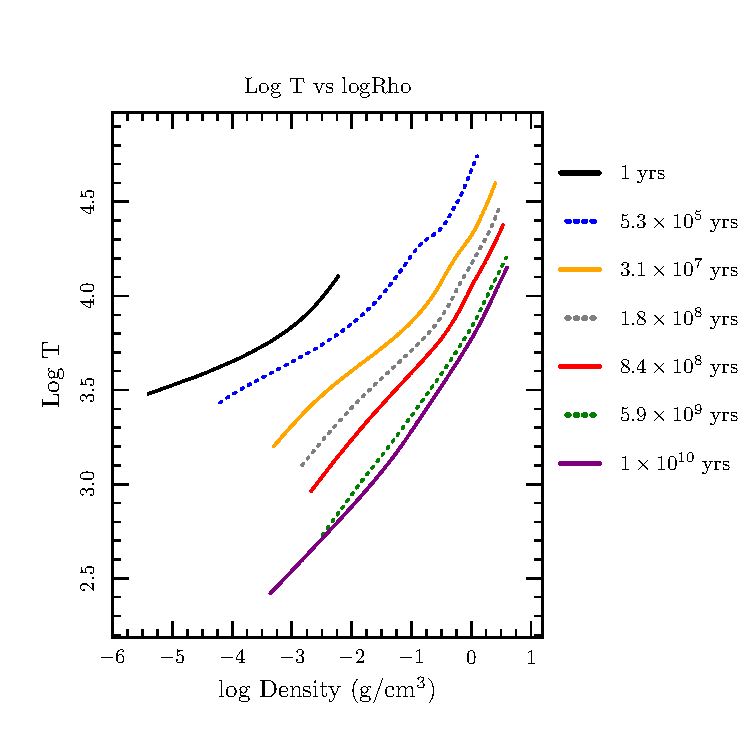
\includegraphics[width = 3.65in]{/Users/jaredbrooks/very_low_mass/plots_out/Log_T_vs_logRho.pdf}
                       \caption{\footnotesize Temperature vs. density profile at a few ages show increase in density and temporary bump in temperature}
                       \label{fig:5}
                \end{minipage}
        \end{figure}

        \pagebreak

        This final plot (figure \ref{fig:6}) shows a few internal \texttt{MESA} variables, such as the size of the time-step, the number of zones, and the number of retries against the model number in order to give some understanding of how hard \texttt{MESA} is working throughout the run and where some areas of problems/interest might be.

        \begin{figure}[H]
                \centering
                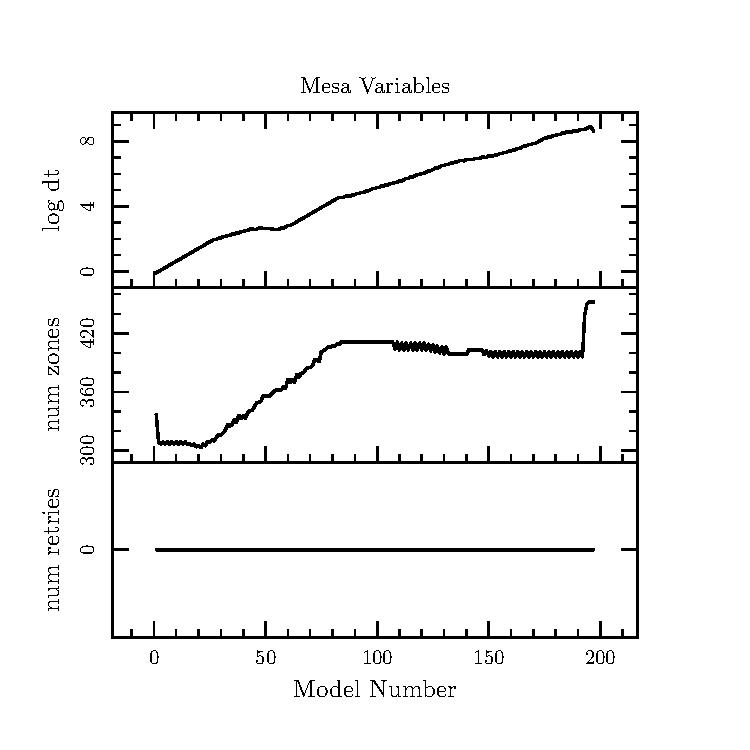
\includegraphics[width = 5in]{/Users/jaredbrooks/very_low_mass/plots_out/Mesa_Variables.pdf}
                \caption{\texttt{MESA} variables plotted against model number show how hard \texttt{MESA} is working}
                \label{fig:6}
        \end{figure}

\end{document}
